\documentclass{article} % For LaTeX2e
\usepackage{iclr2022_conference,times}
% Optional math commands from https://github.com/goodfeli/dlbook_notation.
%%%%% NEW MATH DEFINITIONS %%%%%

\usepackage{amsmath,amsfonts,bm}

% Mark sections of captions for referring to divisions of figures
\newcommand{\figleft}{{\em (Left)}}
\newcommand{\figcenter}{{\em (Center)}}
\newcommand{\figright}{{\em (Right)}}
\newcommand{\figtop}{{\em (Top)}}
\newcommand{\figbottom}{{\em (Bottom)}}
\newcommand{\captiona}{{\em (a)}}
\newcommand{\captionb}{{\em (b)}}
\newcommand{\captionc}{{\em (c)}}
\newcommand{\captiond}{{\em (d)}}

% Highlight a newly defined term
\newcommand{\newterm}[1]{{\bf #1}}


% Figure reference, lower-case.
\def\figref#1{figure~\ref{#1}}
% Figure reference, capital. For start of sentence
\def\Figref#1{Figure~\ref{#1}}
\def\twofigref#1#2{figures \ref{#1} and \ref{#2}}
\def\quadfigref#1#2#3#4{figures \ref{#1}, \ref{#2}, \ref{#3} and \ref{#4}}
% Section reference, lower-case.
\def\secref#1{section~\ref{#1}}
% Section reference, capital.
\def\Secref#1{Section~\ref{#1}}
% Reference to two sections.
\def\twosecrefs#1#2{sections \ref{#1} and \ref{#2}}
% Reference to three sections.
\def\secrefs#1#2#3{sections \ref{#1}, \ref{#2} and \ref{#3}}
% Reference to an equation, lower-case.
\def\eqref#1{equation~\ref{#1}}
% Reference to an equation, upper case
\def\Eqref#1{Equation~\ref{#1}}
% A raw reference to an equation---avoid using if possible
\def\plaineqref#1{\ref{#1}}
% Reference to a chapter, lower-case.
\def\chapref#1{chapter~\ref{#1}}
% Reference to an equation, upper case.
\def\Chapref#1{Chapter~\ref{#1}}
% Reference to a range of chapters
\def\rangechapref#1#2{chapters\ref{#1}--\ref{#2}}
% Reference to an algorithm, lower-case.
\def\algref#1{algorithm~\ref{#1}}
% Reference to an algorithm, upper case.
\def\Algref#1{Algorithm~\ref{#1}}
\def\twoalgref#1#2{algorithms \ref{#1} and \ref{#2}}
\def\Twoalgref#1#2{Algorithms \ref{#1} and \ref{#2}}
% Reference to a part, lower case
\def\partref#1{part~\ref{#1}}
% Reference to a part, upper case
\def\Partref#1{Part~\ref{#1}}
\def\twopartref#1#2{parts \ref{#1} and \ref{#2}}

\def\ceil#1{\lceil #1 \rceil}
\def\floor#1{\lfloor #1 \rfloor}
\def\1{\bm{1}}
\newcommand{\train}{\mathcal{D}}
\newcommand{\valid}{\mathcal{D_{\mathrm{valid}}}}
\newcommand{\test}{\mathcal{D_{\mathrm{test}}}}

\def\eps{{\epsilon}}


% Random variables
\def\reta{{\textnormal{$\eta$}}}
\def\ra{{\textnormal{a}}}
\def\rb{{\textnormal{b}}}
\def\rc{{\textnormal{c}}}
\def\rd{{\textnormal{d}}}
\def\re{{\textnormal{e}}}
\def\rf{{\textnormal{f}}}
\def\rg{{\textnormal{g}}}
\def\rh{{\textnormal{h}}}
\def\ri{{\textnormal{i}}}
\def\rj{{\textnormal{j}}}
\def\rk{{\textnormal{k}}}
\def\rl{{\textnormal{l}}}
% rm is already a command, just don't name any random variables m
\def\rn{{\textnormal{n}}}
\def\ro{{\textnormal{o}}}
\def\rp{{\textnormal{p}}}
\def\rq{{\textnormal{q}}}
\def\rr{{\textnormal{r}}}
\def\rs{{\textnormal{s}}}
\def\rt{{\textnormal{t}}}
\def\ru{{\textnormal{u}}}
\def\rv{{\textnormal{v}}}
\def\rw{{\textnormal{w}}}
\def\rx{{\textnormal{x}}}
\def\ry{{\textnormal{y}}}
\def\rz{{\textnormal{z}}}

% Random vectors
\def\rvepsilon{{\mathbf{\epsilon}}}
\def\rvtheta{{\mathbf{\theta}}}
\def\rva{{\mathbf{a}}}
\def\rvb{{\mathbf{b}}}
\def\rvc{{\mathbf{c}}}
\def\rvd{{\mathbf{d}}}
\def\rve{{\mathbf{e}}}
\def\rvf{{\mathbf{f}}}
\def\rvg{{\mathbf{g}}}
\def\rvh{{\mathbf{h}}}
\def\rvu{{\mathbf{i}}}
\def\rvj{{\mathbf{j}}}
\def\rvk{{\mathbf{k}}}
\def\rvl{{\mathbf{l}}}
\def\rvm{{\mathbf{m}}}
\def\rvn{{\mathbf{n}}}
\def\rvo{{\mathbf{o}}}
\def\rvp{{\mathbf{p}}}
\def\rvq{{\mathbf{q}}}
\def\rvr{{\mathbf{r}}}
\def\rvs{{\mathbf{s}}}
\def\rvt{{\mathbf{t}}}
\def\rvu{{\mathbf{u}}}
\def\rvv{{\mathbf{v}}}
\def\rvw{{\mathbf{w}}}
\def\rvx{{\mathbf{x}}}
\def\rvy{{\mathbf{y}}}
\def\rvz{{\mathbf{z}}}

% Elements of random vectors
\def\erva{{\textnormal{a}}}
\def\ervb{{\textnormal{b}}}
\def\ervc{{\textnormal{c}}}
\def\ervd{{\textnormal{d}}}
\def\erve{{\textnormal{e}}}
\def\ervf{{\textnormal{f}}}
\def\ervg{{\textnormal{g}}}
\def\ervh{{\textnormal{h}}}
\def\ervi{{\textnormal{i}}}
\def\ervj{{\textnormal{j}}}
\def\ervk{{\textnormal{k}}}
\def\ervl{{\textnormal{l}}}
\def\ervm{{\textnormal{m}}}
\def\ervn{{\textnormal{n}}}
\def\ervo{{\textnormal{o}}}
\def\ervp{{\textnormal{p}}}
\def\ervq{{\textnormal{q}}}
\def\ervr{{\textnormal{r}}}
\def\ervs{{\textnormal{s}}}
\def\ervt{{\textnormal{t}}}
\def\ervu{{\textnormal{u}}}
\def\ervv{{\textnormal{v}}}
\def\ervw{{\textnormal{w}}}
\def\ervx{{\textnormal{x}}}
\def\ervy{{\textnormal{y}}}
\def\ervz{{\textnormal{z}}}

% Random matrices
\def\rmA{{\mathbf{A}}}
\def\rmB{{\mathbf{B}}}
\def\rmC{{\mathbf{C}}}
\def\rmD{{\mathbf{D}}}
\def\rmE{{\mathbf{E}}}
\def\rmF{{\mathbf{F}}}
\def\rmG{{\mathbf{G}}}
\def\rmH{{\mathbf{H}}}
\def\rmI{{\mathbf{I}}}
\def\rmJ{{\mathbf{J}}}
\def\rmK{{\mathbf{K}}}
\def\rmL{{\mathbf{L}}}
\def\rmM{{\mathbf{M}}}
\def\rmN{{\mathbf{N}}}
\def\rmO{{\mathbf{O}}}
\def\rmP{{\mathbf{P}}}
\def\rmQ{{\mathbf{Q}}}
\def\rmR{{\mathbf{R}}}
\def\rmS{{\mathbf{S}}}
\def\rmT{{\mathbf{T}}}
\def\rmU{{\mathbf{U}}}
\def\rmV{{\mathbf{V}}}
\def\rmW{{\mathbf{W}}}
\def\rmX{{\mathbf{X}}}
\def\rmY{{\mathbf{Y}}}
\def\rmZ{{\mathbf{Z}}}

% Elements of random matrices
\def\ermA{{\textnormal{A}}}
\def\ermB{{\textnormal{B}}}
\def\ermC{{\textnormal{C}}}
\def\ermD{{\textnormal{D}}}
\def\ermE{{\textnormal{E}}}
\def\ermF{{\textnormal{F}}}
\def\ermG{{\textnormal{G}}}
\def\ermH{{\textnormal{H}}}
\def\ermI{{\textnormal{I}}}
\def\ermJ{{\textnormal{J}}}
\def\ermK{{\textnormal{K}}}
\def\ermL{{\textnormal{L}}}
\def\ermM{{\textnormal{M}}}
\def\ermN{{\textnormal{N}}}
\def\ermO{{\textnormal{O}}}
\def\ermP{{\textnormal{P}}}
\def\ermQ{{\textnormal{Q}}}
\def\ermR{{\textnormal{R}}}
\def\ermS{{\textnormal{S}}}
\def\ermT{{\textnormal{T}}}
\def\ermU{{\textnormal{U}}}
\def\ermV{{\textnormal{V}}}
\def\ermW{{\textnormal{W}}}
\def\ermX{{\textnormal{X}}}
\def\ermY{{\textnormal{Y}}}
\def\ermZ{{\textnormal{Z}}}

% Vectors
\def\vzero{{\bm{0}}}
\def\vone{{\bm{1}}}
\def\vmu{{\bm{\mu}}}
\def\vtheta{{\bm{\theta}}}
\def\va{{\bm{a}}}
\def\vb{{\bm{b}}}
\def\vc{{\bm{c}}}
\def\vd{{\bm{d}}}
\def\ve{{\bm{e}}}
\def\vf{{\bm{f}}}
\def\vg{{\bm{g}}}
\def\vh{{\bm{h}}}
\def\vi{{\bm{i}}}
\def\vj{{\bm{j}}}
\def\vk{{\bm{k}}}
\def\vl{{\bm{l}}}
\def\vm{{\bm{m}}}
\def\vn{{\bm{n}}}
\def\vo{{\bm{o}}}
\def\vp{{\bm{p}}}
\def\vq{{\bm{q}}}
\def\vr{{\bm{r}}}
\def\vs{{\bm{s}}}
\def\vt{{\bm{t}}}
\def\vu{{\bm{u}}}
\def\vv{{\bm{v}}}
\def\vw{{\bm{w}}}
\def\vx{{\bm{x}}}
\def\vy{{\bm{y}}}
\def\vz{{\bm{z}}}

% Elements of vectors
\def\evalpha{{\alpha}}
\def\evbeta{{\beta}}
\def\evepsilon{{\epsilon}}
\def\evlambda{{\lambda}}
\def\evomega{{\omega}}
\def\evmu{{\mu}}
\def\evpsi{{\psi}}
\def\evsigma{{\sigma}}
\def\evtheta{{\theta}}
\def\eva{{a}}
\def\evb{{b}}
\def\evc{{c}}
\def\evd{{d}}
\def\eve{{e}}
\def\evf{{f}}
\def\evg{{g}}
\def\evh{{h}}
\def\evi{{i}}
\def\evj{{j}}
\def\evk{{k}}
\def\evl{{l}}
\def\evm{{m}}
\def\evn{{n}}
\def\evo{{o}}
\def\evp{{p}}
\def\evq{{q}}
\def\evr{{r}}
\def\evs{{s}}
\def\evt{{t}}
\def\evu{{u}}
\def\evv{{v}}
\def\evw{{w}}
\def\evx{{x}}
\def\evy{{y}}
\def\evz{{z}}

% Matrix
\def\mA{{\bm{A}}}
\def\mB{{\bm{B}}}
\def\mC{{\bm{C}}}
\def\mD{{\bm{D}}}
\def\mE{{\bm{E}}}
\def\mF{{\bm{F}}}
\def\mG{{\bm{G}}}
\def\mH{{\bm{H}}}
\def\mI{{\bm{I}}}
\def\mJ{{\bm{J}}}
\def\mK{{\bm{K}}}
\def\mL{{\bm{L}}}
\def\mM{{\bm{M}}}
\def\mN{{\bm{N}}}
\def\mO{{\bm{O}}}
\def\mP{{\bm{P}}}
\def\mQ{{\bm{Q}}}
\def\mR{{\bm{R}}}
\def\mS{{\bm{S}}}
\def\mT{{\bm{T}}}
\def\mU{{\bm{U}}}
\def\mV{{\bm{V}}}
\def\mW{{\bm{W}}}
\def\mX{{\bm{X}}}
\def\mY{{\bm{Y}}}
\def\mZ{{\bm{Z}}}
\def\mBeta{{\bm{\beta}}}
\def\mPhi{{\bm{\Phi}}}
\def\mLambda{{\bm{\Lambda}}}
\def\mSigma{{\bm{\Sigma}}}

% Tensor
\DeclareMathAlphabet{\mathsfit}{\encodingdefault}{\sfdefault}{m}{sl}
\SetMathAlphabet{\mathsfit}{bold}{\encodingdefault}{\sfdefault}{bx}{n}
\newcommand{\tens}[1]{\bm{\mathsfit{#1}}}
\def\tA{{\tens{A}}}
\def\tB{{\tens{B}}}
\def\tC{{\tens{C}}}
\def\tD{{\tens{D}}}
\def\tE{{\tens{E}}}
\def\tF{{\tens{F}}}
\def\tG{{\tens{G}}}
\def\tH{{\tens{H}}}
\def\tI{{\tens{I}}}
\def\tJ{{\tens{J}}}
\def\tK{{\tens{K}}}
\def\tL{{\tens{L}}}
\def\tM{{\tens{M}}}
\def\tN{{\tens{N}}}
\def\tO{{\tens{O}}}
\def\tP{{\tens{P}}}
\def\tQ{{\tens{Q}}}
\def\tR{{\tens{R}}}
\def\tS{{\tens{S}}}
\def\tT{{\tens{T}}}
\def\tU{{\tens{U}}}
\def\tV{{\tens{V}}}
\def\tW{{\tens{W}}}
\def\tX{{\tens{X}}}
\def\tY{{\tens{Y}}}
\def\tZ{{\tens{Z}}}


% Graph
\def\gA{{\mathcal{A}}}
\def\gB{{\mathcal{B}}}
\def\gC{{\mathcal{C}}}
\def\gD{{\mathcal{D}}}
\def\gE{{\mathcal{E}}}
\def\gF{{\mathcal{F}}}
\def\gG{{\mathcal{G}}}
\def\gH{{\mathcal{H}}}
\def\gI{{\mathcal{I}}}
\def\gJ{{\mathcal{J}}}
\def\gK{{\mathcal{K}}}
\def\gL{{\mathcal{L}}}
\def\gM{{\mathcal{M}}}
\def\gN{{\mathcal{N}}}
\def\gO{{\mathcal{O}}}
\def\gP{{\mathcal{P}}}
\def\gQ{{\mathcal{Q}}}
\def\gR{{\mathcal{R}}}
\def\gS{{\mathcal{S}}}
\def\gT{{\mathcal{T}}}
\def\gU{{\mathcal{U}}}
\def\gV{{\mathcal{V}}}
\def\gW{{\mathcal{W}}}
\def\gX{{\mathcal{X}}}
\def\gY{{\mathcal{Y}}}
\def\gZ{{\mathcal{Z}}}

% Sets
\def\sA{{\mathbb{A}}}
\def\sB{{\mathbb{B}}}
\def\sC{{\mathbb{C}}}
\def\sD{{\mathbb{D}}}
% Don't use a set called E, because this would be the same as our symbol
% for expectation.
\def\sF{{\mathbb{F}}}
\def\sG{{\mathbb{G}}}
\def\sH{{\mathbb{H}}}
\def\sI{{\mathbb{I}}}
\def\sJ{{\mathbb{J}}}
\def\sK{{\mathbb{K}}}
\def\sL{{\mathbb{L}}}
\def\sM{{\mathbb{M}}}
\def\sN{{\mathbb{N}}}
\def\sO{{\mathbb{O}}}
\def\sP{{\mathbb{P}}}
\def\sQ{{\mathbb{Q}}}
\def\sR{{\mathbb{R}}}
\def\sS{{\mathbb{S}}}
\def\sT{{\mathbb{T}}}
\def\sU{{\mathbb{U}}}
\def\sV{{\mathbb{V}}}
\def\sW{{\mathbb{W}}}
\def\sX{{\mathbb{X}}}
\def\sY{{\mathbb{Y}}}
\def\sZ{{\mathbb{Z}}}

% Entries of a matrix
\def\emLambda{{\Lambda}}
\def\emA{{A}}
\def\emB{{B}}
\def\emC{{C}}
\def\emD{{D}}
\def\emE{{E}}
\def\emF{{F}}
\def\emG{{G}}
\def\emH{{H}}
\def\emI{{I}}
\def\emJ{{J}}
\def\emK{{K}}
\def\emL{{L}}
\def\emM{{M}}
\def\emN{{N}}
\def\emO{{O}}
\def\emP{{P}}
\def\emQ{{Q}}
\def\emR{{R}}
\def\emS{{S}}
\def\emT{{T}}
\def\emU{{U}}
\def\emV{{V}}
\def\emW{{W}}
\def\emX{{X}}
\def\emY{{Y}}
\def\emZ{{Z}}
\def\emSigma{{\Sigma}}

% entries of a tensor
% Same font as tensor, without \bm wrapper
\newcommand{\etens}[1]{\mathsfit{#1}}
\def\etLambda{{\etens{\Lambda}}}
\def\etA{{\etens{A}}}
\def\etB{{\etens{B}}}
\def\etC{{\etens{C}}}
\def\etD{{\etens{D}}}
\def\etE{{\etens{E}}}
\def\etF{{\etens{F}}}
\def\etG{{\etens{G}}}
\def\etH{{\etens{H}}}
\def\etI{{\etens{I}}}
\def\etJ{{\etens{J}}}
\def\etK{{\etens{K}}}
\def\etL{{\etens{L}}}
\def\etM{{\etens{M}}}
\def\etN{{\etens{N}}}
\def\etO{{\etens{O}}}
\def\etP{{\etens{P}}}
\def\etQ{{\etens{Q}}}
\def\etR{{\etens{R}}}
\def\etS{{\etens{S}}}
\def\etT{{\etens{T}}}
\def\etU{{\etens{U}}}
\def\etV{{\etens{V}}}
\def\etW{{\etens{W}}}
\def\etX{{\etens{X}}}
\def\etY{{\etens{Y}}}
\def\etZ{{\etens{Z}}}

% The true underlying data generating distribution
\newcommand{\pdata}{p_{\rm{data}}}
% The empirical distribution defined by the training set
\newcommand{\ptrain}{\hat{p}_{\rm{data}}}
\newcommand{\Ptrain}{\hat{P}_{\rm{data}}}
% The model distribution
\newcommand{\pmodel}{p_{\rm{model}}}
\newcommand{\Pmodel}{P_{\rm{model}}}
\newcommand{\ptildemodel}{\tilde{p}_{\rm{model}}}
% Stochastic autoencoder distributions
\newcommand{\pencode}{p_{\rm{encoder}}}
\newcommand{\pdecode}{p_{\rm{decoder}}}
\newcommand{\precons}{p_{\rm{reconstruct}}}

\newcommand{\laplace}{\mathrm{Laplace}} % Laplace distribution

\newcommand{\E}{\mathbb{E}}
\newcommand{\Ls}{\mathcal{L}}
\newcommand{\R}{\mathbb{R}}
\newcommand{\emp}{\tilde{p}}
\newcommand{\lr}{\alpha}
\newcommand{\reg}{\lambda}
\newcommand{\rect}{\mathrm{rectifier}}
\newcommand{\softmax}{\mathrm{softmax}}
\newcommand{\sigmoid}{\sigma}
\newcommand{\softplus}{\zeta}
\newcommand{\KL}{D_{\mathrm{KL}}}
\newcommand{\Var}{\mathrm{Var}}
\newcommand{\standarderror}{\mathrm{SE}}
\newcommand{\Cov}{\mathrm{Cov}}
% Wolfram Mathworld says $L^2$ is for function spaces and $\ell^2$ is for vectors
% But then they seem to use $L^2$ for vectors throughout the site, and so does
% wikipedia.
\newcommand{\normlzero}{L^0}
\newcommand{\normlone}{L^1}
\newcommand{\normltwo}{L^2}
\newcommand{\normlp}{L^p}
\newcommand{\normmax}{L^\infty}

\newcommand{\parents}{Pa} % See usage in notation.tex. Chosen to match Daphne's book.

\DeclareMathOperator*{\argmax}{arg\,max}
\DeclareMathOperator*{\argmin}{arg\,min}

\DeclareMathOperator{\sign}{sign}
\DeclareMathOperator{\Tr}{Tr}
\let\ab\allowbreak


%######## APS360: Uncomment your submission name
\newcommand{\apsname}{Project Proposal}
%\newcommand{\apsname}{Progress Report}
%\newcommand{\apsname}{Final Report}

%######## APS360: Put your Group Number here
\newcommand{\gpnumber}{20}

\usepackage{hyperref}
\usepackage{url}
\usepackage{graphicx}
\usepackage{enumitem}
\usepackage{float}


%######## APS360: Put your project Title here
\title{Poetry Through Propogation,\ Generating Haikus With Deep Learning Recurrent Neural Networks}


%######## APS360: Put your names, student IDs and Emails here
\author{Evan Banerjee  \\
Student\# 1009682309\\
\texttt{evan.banerjee@mail.utoronto.ca} \\
\And
Diego Ciudad Real Escalante  \\
Student\# 1009345308 \\
\texttt{diego.ciudadrealescalante@mail.utoronto.ca} \\
\AND
Noah Monti  \\
Student\# 1009452398 \\
\texttt{noah.monti@mail.utoronto.ca} \\
\And
Ji Hong Sayo \\
Student\# 1007314728 \\
\texttt{ji.sayo@mail.utoronto.ca} \\
}

% The \author macro works with any number of authors. There are two commands
% used to separate the names and addresses of multiple authors: \And and \AND.

% Using \And between authors leaves it to \LaTeX{} to determine where to break
% the lines. Using \AND forces a linebreak at that point. So, if \LaTeX{}
% puts 3 of 4 authors names on the first line, and the last on the second
% line, try using \AND instead of \And before the third author name.

\newcommand{\fix}{\marginpar{FIX}}
\newcommand{\new}{\marginpar{NEW}}

\iclrfinalcopy 
%######## APS360: Document starts here
\begin{document}


\maketitle

\begin{abstract}
This is our project proposal for our APS360 final project. We propose building a Recurrent Neural Network that generates Haikus. We will train our model on haiku data from Kaggle, and we will base the architecture off pre-existing deep learning models that have proven successful in generating poetry in the past\\%######## APS360: Do not change the next line. This shows your Main body page count.
----Total Pages: \pageref{last_page}
\end{abstract}



% \section{Project Document Submission for APS360 Course}


% The format for the submissions is a variant of the ICLR 2022 format.
% Please read carefully the instructions below, and follow them
% faithfully. There is a \textbf{9 page} limit for the main text. References do not have any limitation. This is also ICLR's standard length for a paper submission. 
% If your main text goes to page 10, a $-20\%$ penalty would be applied. If your main text goes to page 11, you will not receive any grade for your submission. 

% \subsection{Style}

% Papers to be submitted to APS360 must be prepared according to the
% instructions presented here.

% Authors are required to use the APS360 \LaTeX{} style files obtainable at the
% APS360 website on Quercus. Tweaking the style is not permitted.

% \subsection{Retrieval of style files}

% The file \verb+APS360_Project.pdf+ contains these
% instructions and illustrates the various formatting requirements your APS360 paper must satisfy.
% Submissions must be made using \LaTeX{} and the style files
% \verb+iclr2022_conference.sty+ and \verb+iclr2022_conference.bst+ (to be used with \LaTeX{}2e). The file
% \verb+APS360_Project.tex+ may be used as a ``shell'' for writing your paper. All you have to do is replace the author, title, abstract, and text of the paper with
% your own.

% The formatting instructions contained in these style files are summarized in
% sections \ref{gen_inst}, \ref{headings}, and \ref{others} below.

% \section{General formatting instructions}
% \label{gen_inst}

% The text must be confined within a rectangle 5.5~inches (33~picas) wide and
% 9~inches (54~picas) long. The left margin is 1.5~inch (9~picas).
% Use 10~point type with a vertical spacing of 11~points. Times New Roman is the
% preferred typeface throughout. Paragraphs are separated by 1/2~line space,
% with no indentation.

% Paper title is 17~point, in small caps and left-aligned.
% All pages should start at 1~inch (6~picas) from the top of the page.

% Authors' names are
% set in boldface, and each name is placed above its corresponding
% address. The lead author's name is to be listed first, and
% the co-authors' names are set to follow. Authors sharing the
% same address can be on the same line.

% Please pay special attention to the instructions in section \ref{others}
% regarding figures, tables, acknowledgments, and references.


% There will be a strict upper limit of 9 pages for the main text of the initial submission, with unlimited additional pages for citations. 

% \section{Headings: first level}
% \label{headings}

% First level headings are in small caps,
% flush left and in point size 12. One line space before the first level
% heading and 1/2~line space after the first level heading.

% \subsection{Headings: second level}

% Second level headings are in small caps,
% flush left and in point size 10. One line space before the second level
% heading and 1/2~line space after the second level heading.

% \subsubsection{Headings: third level}

% Third level headings are in small caps,
% flush left and in point size 10. One line space before the third level
% heading and 1/2~line space after the third level heading.

% \section{Citations, figures, tables, references}
% \label{others}

% These instructions apply to everyone, regardless of the formatter being used.

% \subsection{Citations within the text}

% Citations within the text should be based on the \texttt{natbib} package
% and include the authors' last names and year (with the ``et~al.'' construct
% for more than two authors). When the authors or the publication are
% included in the sentence, the citation should not be in parenthesis using \verb|\citet{}| (as
% in ``See \citet{Hinton06} for more information.''). Otherwise, the citation
% should be in parenthesis using \verb|\citep{}| (as in ``Deep learning shows promise to make progress
% towards AI~\citep{Bengio+chapter2007}.'').

% The corresponding references are to be listed in alphabetical order of
% authors, in the \textsc{References} section. As to the format of the
% references themselves, any style is acceptable as long as it is used
% consistently.

% To cite a new paper, first, you need to add that paper's BibTeX information to \verb+APS360_ref.bib+ file and then you can use the \verb|\citep{}| command to cite that in your main document. 

% \subsection{Footnotes}

% Indicate footnotes with a number\footnote{Sample of the first footnote} in the
% text. Place the footnotes at the bottom of the page on which they appear.
% Precede the footnote with a horizontal rule of 2~inches
% (12~picas).\footnote{Sample of the second footnote}

% \subsection{Figures}

% All artwork must be neat, clean, and legible. Lines should be dark
% enough for purposes of reproduction; art work should not be
% hand-drawn. The figure number and caption always appear after the
% figure. Place one line space before the figure caption, and one line
% space after the figure. The figure caption is lower case (except for
% first word and proper nouns); figures are numbered consecutively.

% Make sure the figure caption does not get separated from the figure.
% Leave sufficient space to avoid splitting the figure and figure caption.

% You may use color figures.
% However, it is best for the
% figure captions and the paper body to make sense if the paper is printed
% either in black/white or in color.

% \begin{figure}[h]
% \begin{center}
% 
\includegraphics[width=0.6\textwidth]{Figs/td-deep-learning.jpg}
% \end{center}
% \caption{Sample figure caption. Image: ZDNet}
% \end{figure}

% \subsection{Tables}

% All tables must be centered, neat, clean and legible. Do not use hand-drawn
% tables. The table number and title always appear before the table. See
% Table~\ref{sample-table}.

% Place one line space before the table title, one line space after the table
% title, and one line space after the table. The table title must be lower case
% (except for first word and proper nouns); tables are numbered consecutively.

% \begin{table}[t]
% \caption{Sample table title}
% \label{sample-table}
% \begin{center}
% \begin{tabular}{ll}
% \multicolumn{1}{c}{\bf PART}  &\multicolumn{1}{c}{\bf DESCRIPTION}
% \\ \hline \\
% Dendrite         &Input terminal \\
% Axon             &Output terminal \\
% Soma             &Cell body (contains cell nucleus) \\
% \end{tabular}
% \end{center}
% \end{table}


\section{Introduction}
“Poetry heals the wounds inflicted by reason” —Novalis\\

In this project we propose to build a deep learning model to generate short poems of various topics. 
Poetry has long been regarded as a deep expression of emotion and human experience. 
Given that the model we construct will possess neither emotions nor intuition, 
we are interested to see whether our construction will be able to imitate human poetry, 
and if so to what degree. If the model is capable of producing compelling poems as output, 
this would contradict the idea that poetry requires emotion to produce, 
with implications for our understanding of the nature of creative work in general.\\

This is a similar technical problem to the one addressed by large language models,
though it is considerably smaller-scale given our limited time and resources. Rather than generating arbitrary text,
we propose to train on and generate only poetry. Focusing on poetry offers technical advantages beyond limiting the scope of the project: 
the rules of grammar and punctuation are generally considered more flexible in poetry than in prose writing,
which may reduce the required complexity of the mode and allow for a wider range of acceptable output.\\

Besides our interest in the philosophical implications of a machine engaging in what many consider a characteristically human activity,
there will also be practical applications for our proposed model.
Generating poetry of different styles may yield new insights on the defining characteristics of each style. 
Additionally, the successes and failures of a neural network trying to generate poetry may uncover novel insights into the structure of different poetic forms and what constitutes ‘good’ poetry for different genres.
As such, our project will help enable human writers to be better poets, while raising interesting questions on the nature of poetic expression and its connections to emotion and consciousness.\\

Our code can be found at this GitHub repository: https://github.com/Evan-Banerjee/aps360




\section{Illustration}
\begin{figure}[h]
    \begin{center}
    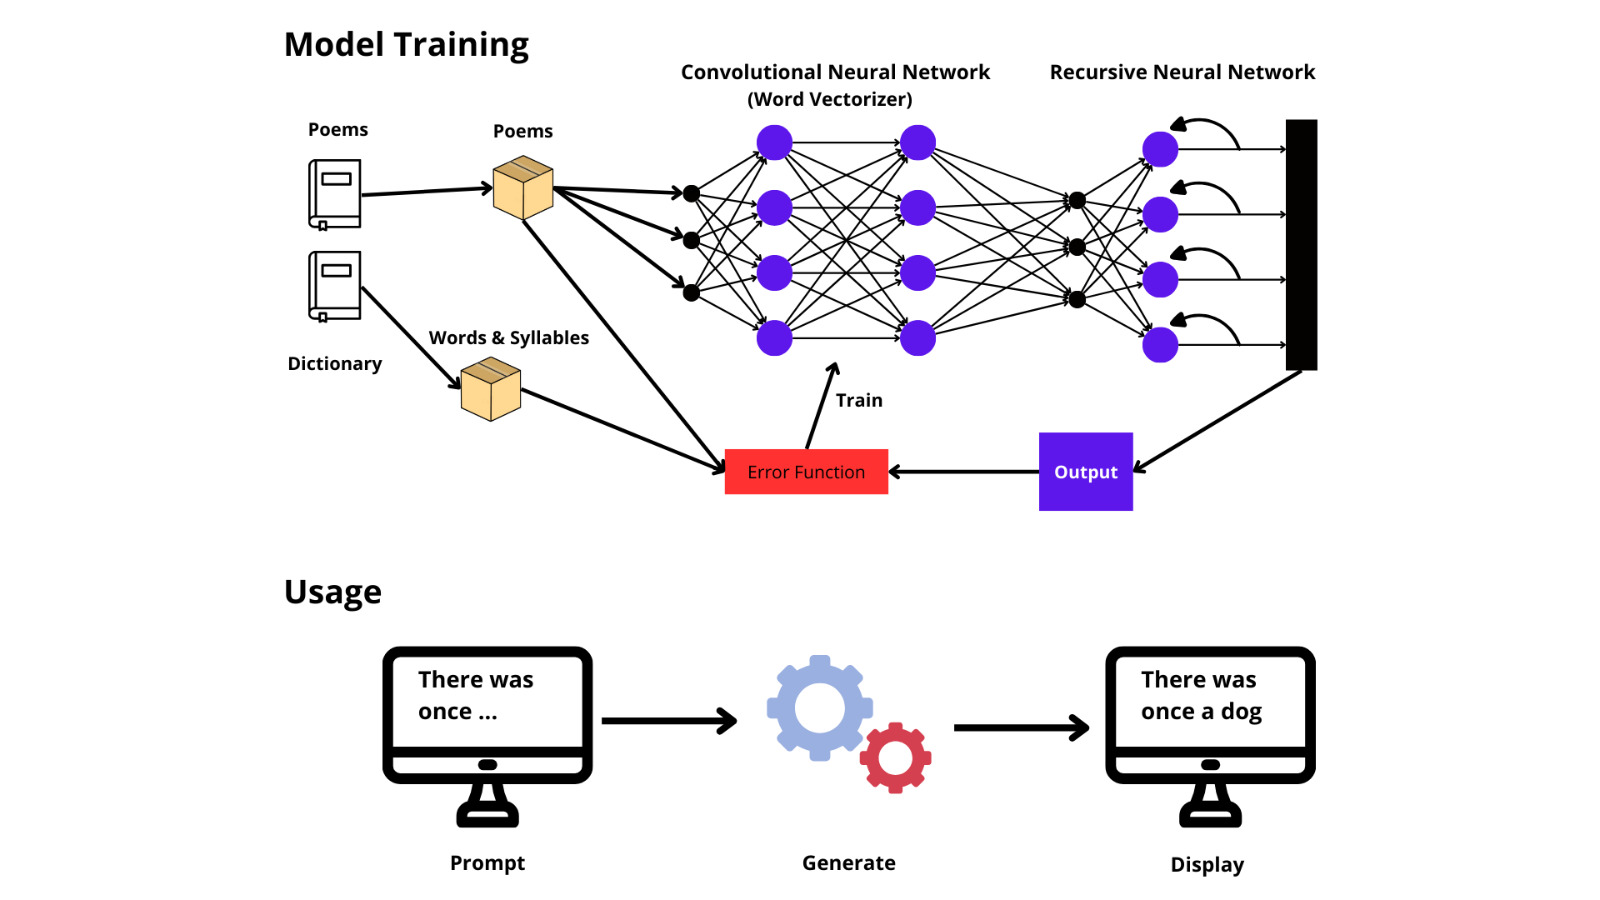
\includegraphics[width=\textwidth]{Figs/Illustration.jpg}
    \end{center}
    \caption{Figure 1: Proposed Model (Training/Deployment)}
    \end{figure}

\section{Background \& Related Work}
Previous poetry generation models utilized Recurrent Neural Networks (RNN) with some form of memory limiting to generate poems off a large dataset.\\\\
One model, created by researchers at the University of Saarland, utilized encoder decoder systems, as well as long short-term memory (LSTM) and Gated Recurrent Units (GRU) to address vanishing gradients, \citep{novikovaenglish}.\\\\
Another model, developed at the University of Edinburgh utilized multiple neural networks chained together, with a convolutional neural network (CNN) for encoding, one RNN for creating hidden context parameters,
and another RNN with a separate weight vector for modifying the final output \citep{zhang2014chinese}.
The output of this model was particularly compelling, with human ratings for the generated poems being over 75\% of the ratings given to human written poems.\\\\
Another model, built at City, University of London, used syllables as the inputs and outputs of their RNN instead of words \citep{lewis2021syllable}.
This model’s poems were incredibly convincing, with 56\% of polled individuals believing the AI generated poems were written by humans.\\\\
When focusing specifically on haikus, even a relatively basic model built by students at Stanford University was able to score well \citep{haikugeneration}. 
For this model human evaluators gave the AI generated haikus an average quality score that was over 80\% of the average score given to human poems. This model only used a single RNN with LSTM. 
Granted, the evaluations were only done by 8 individuals, but the strength of RNNs for this kind of task is evident.\\\\
Finally, a model presented at the 13th conference on language resources and evaluation found a large degree of success in constraining the output of neural networks to generate poems \citep{popescu2022constrained}.
This model forced the AI to repeatedly output lines of a poem until certain syntax requirements were met. 
It also enabled the user to specify emotional tone by encoding category preferences (happy, sad, etc.) into a weighted vector that was then used after generating a line to swap out words that didn’t fit the categories well with words that did.\\\\
This was most effectively done when words were chosen based on word frequency from other poems that fit the specified category. 
This model also utilized a softmax function that truncates the least likely words from the sample space during generation, increasing the probability of likely words and drastically improving output.\\\\
Our model will utilize many of these techniques, though the exact extent is still to be determined.


\section{Data Processing}

The data we have gathered consists of two datasets collected from Kaggle. One contains over 115,000 haikus in English and their meter \citep{Jhalani_2020}. The second one is composed of approximately 130.000 words in the English dictionary \citep{Schwartz_2022} and will serve as a starting point for the language model to gather words from it. From the haiku database, we will only take the ones with a 5-7-5 structure so that we have a more rigid definition of a haiku our model can hopefully learn.  In terms of data processing, we will parse the CSV files and extract the poem’s text and meter. By the end, we will be left with only the haikus who follow the 5-7-5 structure and a list of all the words in the English language along with their syllables.

The data processing of the poems will then follow these steps:

\begin{enumerate}
    \item Remove the unused columns of data.
    \begin{enumerate}[label=\alph*)] % Nested list with lowercase letters
        \item Remove the columns that are not relevant for our purposes. The CSV file for haikus will only have the poem and meter field.
        \item In the dictionary dataset, this means removing all the columns except for “word” and “syllable count”. This dataset is now processed.
    \end{enumerate}
    \item Filter the poems.
    \begin{enumerate}[label=\alph*)]
        \item Remove the rows that contain poems whose tags aren’t related to one of the “genres” we will work on. The related tags are to be manually selected. For the haikus, this removes all the haikus that do not have the 5-7-5 structure.
    \end{enumerate}
\end{enumerate}


\section{Architecture}
For this project, we have chosen the Long Short-Term Memory (LSTM) model, which is based on a Recurrent Neural Network (RNN).\\\\

An LSTM model is a modified version of an RNN that is especially good when it comes to remembering past data that was entered.
One of the issues present in many RNN models is called the vanishing gradient, which occurs when the gradients become extremely small as they are back-propagated during training.
This is can occur due to the activation functions having derivatives less than 1 (or equal to zero in the case of dead neurons using ReLu activations), 
but it can also happen simply because the weights used as coefficients in many of the derivative terms in backpropagation are relatively small, 
so the number of distinct terms in the sum for any one gradient (equal to the number of distinct paths from one node to the output) ends up being exponentially smaller than the size of each individual term.
This is unavoidable if the weights are kept small enough to prevent the opposite problem, where gradients explode due to each individual term not shrinking fast enough to account for the massive increase in terms.
This is especially problematic in RNNs because each new term processed during training essentially creates a new layer, so as time goes on, each chain of partial derivatives decreases exponentially faster than the number of chains increases, and the gradient tends to zero.
LSTM will address this issue by changing the RNN so it doesn’t create new layers.
Instead, a new vector called the cell state will be made, likely with the same dimensionality as the hidden state vector, 
and it will be updated at each time step using forget and input “gates”.
These gates will be separate neural network layers (likely with low depth) that use the new inputs and previous hidden states to increase or decrease certain values in the cell state to represent “forgetting” or “learning” new information.
Then an “output gate”, which is another neural network (of relatively low depth) takes in the modified cell state to calculate the new hidden state, which can be used with the next input to begin the modification process all over again.
These gates have to be trained with backpropagation, and they are limited in the quantity of information they can encode, but they fix the error of vanishing gradients because now the number of layers is constant during training since the “memory” of the training is encoded in a finite vector.\\\\

Beyond using LSTM, our model will incorporate a vectorization algorithm that will originally be a pre-trained Convolutional Neural Network (CNN), but that we may replace with an untrained one that we include in the backpropagation training.
The output of the RNN will be a logit, which we will transform with a softmax function to create a probability distribution to choose the next word in the haiku.
Newline characters will be part of the corpus of words so that the outputted poems span multiple lines.
The softmax function will incorporate truncation into our softmax model to improve word selection.
The network will be forced to output lines multiple times if it fails to meet syntax requirements, and we will algorithmically choose the output that matches our format most closely.
Finally, if time permits, we will incorporate category labels into our training dataset and utilize word frequency lists between categories to dynamically swap out words post-line generation to push the topics in the direction the user specifies.
If possible, we’ll also incorporate this word frequency weighting into the final softmax function to prioritize words that more closely match the theme.


\section{Baseline Model}

We will be comparing our model against a Markov chain based text generation algorithm.
The specific instance we will derive this from is \citep{haikugeneration}.\\\\
Markov-chain based algorithms for text generation were one of the more common methods before neural network based models became a viable option.
By starting with a body of text, the algorithm creates a probability map of which words are most likely to follow one another, 
and through a starting word or phrase, the algorithm recursively finds the most likely word to appear next in a sentence based on the previous word until a desired length is achieved.\\\\
These algorithms are usually simple and highly performant, however, because they are only able to capture local patterns, Markov based algorithms are limited in scope and have a lack of coherence over longer passages. 
Comparing our neural network model against a Markov chain algorithm will demonstrate the difference in sophistication we are able to achieve using a more modern approach, 
and how it changes over various generated passages.


\section{Ethical Considerations}
Despite AI being around for several decades, it was only recently that computational power necessary to generate human-level works of art became widely available. As impressive as they are, Increasingly improving models that generate images, written stories, and poems also raise questions about how these models get and utilize their training data. After all, if a human can learn to imitate another human, what stops a machine from imitating the copyrighted work of an artist?\\\\

While this is a very trending topic, legislation protecting individuals from having their written works used to train AI models is still in early stages which is why we are taking additional caution. We will take several steps to ensure that we are not infringing upon an author’s intellectual property. First, we will be taking our poems from datasets found in Kaggle. This way we can use their terms of services as a moral guideline for how to utilize these datasets \citep{Kaggle_2024}. This means we will not redistribute them as that would constitute plagiarism. Additionally, the poems we will be using list their source of origin. With this, we can be certain that the poems look at come from a publicly accessible source and not copyright-protected material. Finally, this model is a purely academic experiment, and we do not seek to benefit from the material it generates. Therefore, the literary works we will deal with in this project and our use of them fall under fair dealings as per Canadian law \citep{LegislativeServicesBranch_2024}.\\\\

We have discussed the steps that we will take to prevent misuse of our training data, now let’s dig deeper into how someone with harmful intentions might use our project. The biggest cause of concern comes from poem-writing competitions. Instead of having to naturally come up with poems, someone might take advantage of a deep learning model to easily generate several entries, increasing their chances of winning or simply overloading the contest’s submission portal. While many competitions may not explicitly ban AI-generated poems, it is not hard to see how a generated poem winning over many human authors may be seen as controversial. Our system somewhat counteracts this by having the user be vital in the poem creation as they must prompt the model in order for it to generate anything. Additionally, our limited scope of haikus would make it harder for someone to take advantage of the model on a massive scale as haikus are notoriously short.


\section{Project Plan}
\label{project_plan}

\begin{figure}[H]
    \begin{center}
    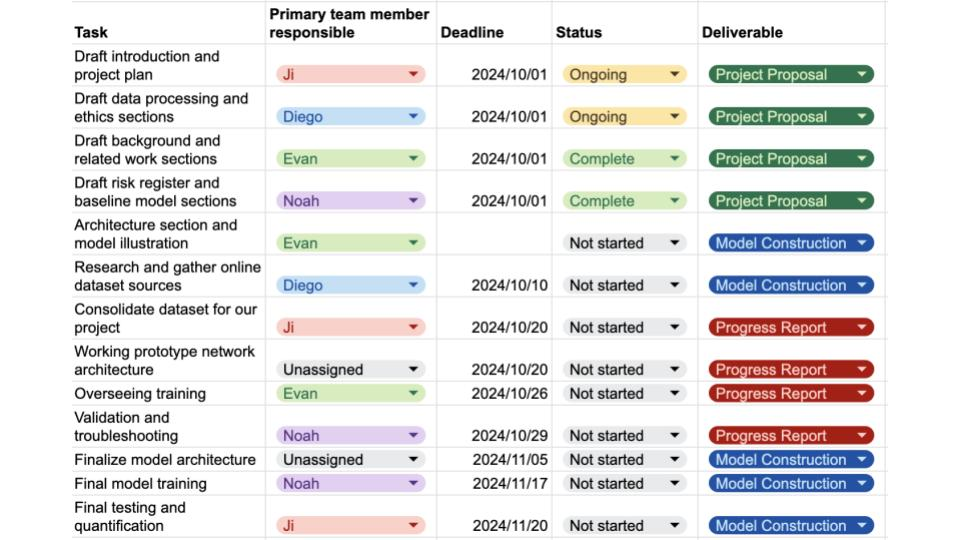
\includegraphics[width=\textwidth]{Figs/project-plan.jpg}
    \end{center}
    \caption{Figure 2: Project Plan}
    \end{figure}

\subsection{Communication}
Team communication will take place via WhatsApp group, which all team members will check daily. We will also hold weekly in-person meetings to discuss task progress after our shared lab session, and asynchronous Zoom meetings as needed for specific tasks and deliverables that require full-team input.

\subsection{Team Norms}
we plan to work in a GitHub repository, which will facilitate version control and ensure no work is lost during editing.\\\\ 
Note: the project plan remains somewhat open, to allow for pivoting as we learn more about the requirements of the project. Also note that the individual task assignments are not absolute, and all team members will collaborate on difficult tasks as needed.


\section{Risk Register}
\label{risk_register}

\subsection{Model does not generate coherent output}

This is possible due to the complexity of generating text, and the potentially large variations in the training data. If our created model is not generating poems that make sense, does not output enough text to be acceptable, or takes too long to generate text, we would first scale back the model to only focus on creating one sentence at a time, and increase the amount of training data it has to work with. Once we have refined our model and see consistent results, we would then increase its size and continuously evaluate its performance as it scales.

\subsection{Team member drops the course}

If a team member decides to drop the course, a meeting will take place where the departing member will go over in detail all of their assigned sections such as: what has been completed, what is in progress, what gave them challenges, etc. Once the team has figured out which parts of the project are affected, the remaining members will meet and see which parts align best with their currently assigned portions and/or expertise. In the event the departing member had a portion that is unrealistic to finish in time, the scope of the project will be re-evaluated.

\subsection{Model is taking too many resources to train}

If the model requires much more time or compute resources to properly train than anticipated, and it is not an issue of improperly constructed code, the team will analyze the individual components of the model to figure out which ones are requiring the largest amount of resources. For example, if the training sets are too large or take too long on our computers, we will first see if we have access to a more powerful computer the training can be performed on. If this is unrealistic or inaccessible, the scope will be re-evaluated in order to have it properly fit within our given resources, which could be reducing complexity of the model or using smaller datasets.

\subsection{Original Scope is too large}

If the realization comes up that we were too ambitious in our original goal, and constraints such as available working time or complexity become large enough issues where in the proposed design is unlikely to be met, each member will share their concerns which could be regarding other commitments such as classes, lack of understanding when it comes to their assigned section, or any other concern that impacts the progress of the project. We will then make any necessary changes to the project design and scope to ensure a working model is delivered.

\subsection{Internal Disagreement about project direction}

If one or more team members brings up any issues they see with the project that could impact progress, a team meeting will take place at which the concerns are communicated to the other members. Each member will have the opportunity to share their opinions on the matter, after which we will deliberate over potential solutions until the entire team feels satisfied with the choices made going forward.


% \section{Final instructions}
% Do not change any aspects of the formatting parameters in the style files.
% In particular, do not modify the width or length of the rectangle the text
% should fit into, and do not change font sizes (except perhaps in the
% \textsc{References} section; see below). Please note that pages should be
% numbered.


% \subsubsection*{Author Contributions}
% If you'd like to, you may include  a section for author contributions as is done
% in many journals. This is optional and at the discretion of the authors.

% \subsubsection*{Acknowledgments}
% Use unnumbered third level headings for the acknowledgments. All
% acknowledgments, including those to funding agencies, go at the end of the paper.
\pagebreak
\label{last_page}

\bibliography{APS360_ref}
\bibliographystyle{iclr2022_conference}

\end{document}
